%% Feedforward Racing-Line Tracking with an Adaptive Clock for Robust Autonomous Drone Racing
%% Built on the IEEE conference template (IEEEtran).
%% Added over the base template: tikz (self-contained figures) and algorithm (pseudocode float).
%% Two image slots are left for you to fill (see \figplaceholder). Compile with pdflatex, run twice.
\documentclass[conference]{IEEEtran}
\IEEEoverridecommandlockouts
% The preceding line is only needed to identify funding in the first footnote. If that is unneeded, please comment it out.
\usepackage{cite}
\usepackage{amsmath,amssymb,amsfonts}
\usepackage{algorithm}
\usepackage{algorithmic}
\usepackage{graphicx}
\usepackage{textcomp}
\usepackage{xcolor}
\usepackage{tikz}
\usetikzlibrary{arrows.meta,positioning,calc,shapes.geometric}
\def\BibTeX{{\rm B\kern-.05em{\sc i\kern-.025em b}\kern-.08em
    T\kern-.1667em\lower.7ex\hbox{E}\kern-.125emX}}

% Image slot to be replaced by a screenshot or a plot. Compiles as a framed grey box.
\newcommand{\figplaceholder}[2]{%
  \setlength{\fboxsep}{0pt}%
  \fcolorbox{gray!60}{gray!8}{\parbox[c][#1][c]{0.98\linewidth}{\centering\small\itshape\textcolor{gray!70}{#2}}}%
}

\begin{document}

\title{Feedforward Racing-Line Tracking with an Adaptive Clock\\ for Robust Autonomous Drone Racing}

\author{\IEEEauthorblockN{1\textsuperscript{st} Ahmet Arda Hız}
\IEEEauthorblockA{\textit{Learning Systems and Robotics} \\
\textit{Technical University of Munich}\\
Munich, Germany \\
aarda.hiz@tum.de}
\and
\IEEEauthorblockN{2\textsuperscript{nd} Deniz \"Ozt\"urk}
\IEEEauthorblockA{\textit{Learning Systems and Robotics} \\
\textit{Technical University of Munich}\\
Munich, Germany \\
deniz.oeztuerk@tum.de}
}

\maketitle

\begin{abstract}
Autonomous drone racing tests a controller at the limit of a vehicle's dynamics. We study the disturbed setting, where gate and obstacle positions are shifted by up to 15 cm and the true values are revealed only when the drone is within 0.7 m. We present a controller that does not run an optimizer in the loop. A time-optimal racing line is built once from the nominal course, and the drone tracks it with a feedforward term and a PD law. Two ideas make this fast and reliable under disturbance. First, the line is not rebuilt when a gate is revealed. It is slid onto the true gate and pushed clear of obstacles, so the shape stays and only the position moves. Second, the drone flies the line by an adaptive clock. Near a gate the clock slows or stops when the drone falls behind, so the drone never reaches a gate ahead of where it can hold the line. On the competition track the controller passes all 20 evaluation runs in simulation with a lap time of 6.89 s. This is faster than an online optimization controller that we flew on the real drone at 9.55 s. We describe the design and report the effect of each part.
\end{abstract}

\section{Introduction}
Autonomous drone racing asks a controller to fly a quadrotor through a set of gates in the shortest time without hitting a gate frame or an obstacle. It is a common benchmark because a fast lap forces the vehicle to work near its actuation limit, where small errors are punished at once \cite{survey}. Much of the drone racing work assumes a known track, where every gate position is fixed before the flight and the task is a single time-optimal trajectory \cite{foehn,minsnap}. A real track breaks that assumption. Gates are placed by hand, they drift and the vehicle only sees the true geometry once it is close.

We study the disturbed setting of the LSY Drone Racing competition. Gate and obstacle positions are drawn from their nominal values with a shift of up to 15 cm, and the true value of an object is reported only when the drone is within 0.7 m of it. A controller that wins here needs two things at once. It has to fly a fast line through the course, and it has to correct for a gate that has moved before it reaches the gate.

Two families of methods lead this task. One solves an optimization at every step, for example Model Predictive Contouring Control (MPCC) \cite{mpcc}. The other learns a policy from data with reinforcement learning \cite{champion,songrl}. Both are strong, and we built an optimization based controller first. It needs a compiled solver in the loop and it was hard to push below eight seconds on this track. We then took a simpler route that turned out faster and more reliable. We build one time-optimal racing line offline and track it. The contribution of this report is that controller and two design choices that make it work under disturbance.
\begin{itemize}
\item The offline line is not rebuilt when a gate is revealed. It is warped: slid onto the true gate with a smooth blend between gates, and pushed clear of obstacles and gate posts.
\item The drone flies the line by an adaptive clock. When it falls behind near a gate the clock slows or stops, so the drone stays centered in the opening.
\end{itemize}
On the competition track the controller passes all 20 evaluation runs in simulation at 6.89 s, faster than our optimization based controller, which we flew on the real drone at 9.55 s.

\section{Related Work}
\label{sec:related}
Time-optimal quadrotor flight through a fixed set of gates is well studied. Foehn et al.\ compute a full time-optimal trajectory that respects the single-rotor thrust limits \cite{foehn}. These methods give the fastest known laps on a known track, but they are expensive and assume the gates do not move, so they do not fit an online disturbed setting on their own.

A cheaper and common pipeline splits the problem into a path and a timing. A geometric path is planned first, then a time-optimal speed profile is placed on it with bounded velocity and acceleration \cite{kunz,verscheure}. Minimum-snap trajectories are a popular choice for the second step \cite{minsnap}. Prior work in this competition reports that minimum snap can leave the collision-free corridor at sharp corners, which is a problem once gates move. We keep the split into a path and a timing, and we use the bounded-acceleration profile rather than minimum snap.

For the online part, MPCC solves a contouring problem at every step and trades speed against tracking inside one optimization \cite{mpcc}. It is powerful and it handles a moving gate by re-solving, but it needs a compiled solver in the loop. Learning based controllers train a policy that maps the observation to an action in one forward pass \cite{champion,songrl}. They reach strong times, but they need training and they are harder to inspect. Our controller sits between the classic pipeline and the online methods. We plan one line offline, and we react to the reveal with a cheap warp and an adaptive clock rather than a new solve.

\section{Problem Description}
\label{sec:problem}
We use the LSY Drone Racing environment, which builds on the safe-control-gym benchmark \cite{scg} with a Crazyflie 2.1 quadrotor \cite{crazyflie} as the model. The vehicle has a mass of 43 g and a thrust to weight ratio near 1.9. The track holds four gates and four obstacles. A gate opening is 0.4 m wide inside a 0.72 m frame, so the usable gap is about three vehicle widths.

At each step the controller reads an observation
\begin{equation}
o = [\, p,\; v,\; q,\; G,\; O,\; i \,],
\label{eq:obs}
\end{equation}
with position $p \in \mathbb{R}^3$, velocity $v \in \mathbb{R}^3$, orientation quaternion $q$, the gate poses $G$, the obstacle positions $O$ and the index $i$ of the next gate. Gate and obstacle positions start at their nominal values and switch to the true value once the drone is within the 0.7 m sensor range. In the lab the true poses come from an external motion capture system Vicon, which tracks reflective markers on the gates and obstacles. The 0.7 m range stands in for the drone's own detection range, so before that the controller uses the nominal pose. The command is sent at 50 Hz. The environment runs in attitude mode, so the output is
\begin{equation}
a = [\, \phi,\; \theta,\; \psi,\; f \,],
\label{eq:act}
\end{equation}
a roll, pitch and yaw with a collective thrust $f$. An onboard controller at 500 Hz tracks $a$. The controller therefore does not set motor forces directly.

Disturbances act on the drone and on the track. The drone mass, inertia and start pose are perturbed at every reset, and noise is added to the dynamics. Gate positions are shifted by up to 15 cm and their yaw is rotated. Obstacle positions are shifted by up to 15 cm. The score for a run is the time to pass the final gate. A run is a success if the drone passes all gates in order without a collision and without leaving the arena.

The challenge is organized as a ladder of difficulty levels that differ by which disturbances are active. Level 0 has no disturbance. The drone and the full track are known, so it measures raw speed. Level 1 randomizes the drone's inertial properties, its mass and inertia, and its start pose, while the track stays known. Level 2 also randomizes the gate and obstacle poses within the bounds above, revealed within the sensor range, on a layout that is otherwise fixed. Level 3 randomizes the layout itself, so the gate positions and the gate order change every run, which needs planning from scratch in flight. The final evaluation uses a separate configuration, \texttt{final.toml}, provided in the last lab session. It keeps the drone and pose disturbances, up to 15 cm on each gate and obstacle revealed within 0.7 m, but it fixes the nominal gate and obstacle layout. This is deliberate. Every group flies the same fixed course, so the lap times compare directly across groups. The fixed layout is also what lets our controller build its racing line offline.

One feature of the setting drives the whole design. A gate is seen late. A gate that has moved by 15 cm is revealed at 0.7 m, and the drone has a short window to move onto the new opening. The faster it flies, the less time it has for that correction. This links speed to the risk of a miss and sets the trade the controller has to manage.

\section{Methodology}
\label{sec:method}

\subsection{Overview}
The controller has an offline part and an online part, shown in Fig.~\ref{fig:pipeline}. Once, at the end of takeoff, it builds a time-optimal racing line from the nominal gates. From then on it runs a fixed loop at 50 Hz. It reads the observation, warps the stored line onto the revealed gates and obstacles, advances an adaptive clock and returns a feedforward acceleration corrected by a PD law. The line itself is never rebuilt. There is no optimizer in the loop.

\begin{figure}[t]
\centering
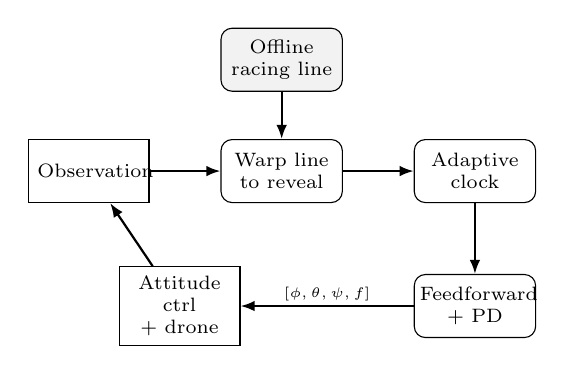
\begin{tikzpicture}[
  node distance=6mm and 9mm,
  block/.style={draw, rounded corners, align=center, minimum height=8mm, inner sep=2pt, font=\scriptsize, text width=14mm},
  io/.style={draw, align=center, font=\scriptsize, text width=13mm, minimum height=8mm},
  arr/.style={-{Latex[length=1.8mm]}, thick}
]
\node[io] (obs) {Observation};
\node[block, right=of obs] (warp) {Warp line\\ to reveal};
\node[block, right=of warp] (clock) {Adaptive\\ clock};
\node[block, below=9mm of clock] (track) {Feedforward\\ + PD};
\node[io, left=22mm of track] (drone) {Attitude ctrl\\ + drone};
\node[block, above=6mm of warp, fill=gray!10] (line) {Offline\\ racing line};

\draw[arr] (line) -- (warp);
\draw[arr] (obs) -- (warp);
\draw[arr] (warp) -- (clock);
\draw[arr] (clock) -- (track);
\draw[arr] (track) -- node[midway, above, font=\tiny, fill=white, inner sep=1.5pt]{$[\phi,\theta,\psi,f]$} (drone);
\draw[arr] (drone) -- (obs);
\end{tikzpicture}
\caption{Controller structure. The racing line is built once (grey block) and stored. Each step the line is warped onto the revealed gates and obstacles, an adaptive clock picks the current reference point and a feedforward plus PD law produces the attitude command.}
\label{fig:pipeline}
\end{figure}

\subsection{The Racing Line}
\label{sec:line}
The line is a smooth curve through the four gates. We first place waypoints. Let $g_j$ be a gate center and $n_j$ its facing direction in the plane. For each gate we add an entry point and an exit point on the facing axis,
\begin{equation}
e_j = g_j - d_{\text{pre},j}\, n_j, \qquad x_j = g_j + d_{\text{post},j}\, n_j,
\label{eq:entryexit}
\end{equation}
and two close knots at $g_j \pm 0.1\, n_j$ that bracket the center. The close knots force the spline to cross the opening along the facing axis, so the drone goes straight through the gate and not at an angle. When the gap between two gates is large we add one control point on the leg, offset from the straight midpoint, so the curve keeps a wide and low-curvature shape. Points that fall within 6 cm of a neighbor are dropped, which keeps the spline well conditioned.

The waypoints are joined by a clamped cubic spline. It is twice differentiable and gives a smooth position, velocity and acceleration. The clamped end condition lets the line start along the current velocity at takeoff, so the drone leaves the climb with momentum along the line. The offsets $d_{\text{pre},j}$, $d_{\text{post},j}$ and the leg control points are tuned once offline for this track.

\subsection{Time-Optimal Speed Profile}
\label{sec:speed}
The spline sets the shape. A speed profile sets how fast to fly it. We use the standard time-optimal path parametrization \cite{kunz,verscheure}. The drone has one acceleration budget, and it is shared between turning and speeding up. In a tight turn most of the budget holds the vehicle in the turn, so the speed there is low. On a straight the budget is free for acceleration, so the speed there is high.

Let $s$ be the arc length, $\kappa(s)$ the path curvature and $v(s)$ the speed. We build the profile in three passes. First a curvature cap from the turning budget $a_{\text{lat}}$ and a top speed $v_{\text{ceil}}$,
\begin{equation}
v_{\text{cap}}(s) = \min\!\left( \sqrt{a_{\text{lat}} / \kappa(s)},\; v_{\text{ceil}} \right).
\label{eq:curv}
\end{equation}
We also cap the speed inside a small radius of each gate, so the crossing is slow enough to stay centered. Second a forward pass. At each step the lateral share of the budget is $a_{\text{lat}} = \kappa\, v^2$, and the rest is free to speed up. With a forward budget $a_H$ the speed can rise by
\begin{equation}
v_{i+1} \le \sqrt{\, v_i^2 + 2\,\Delta s_i\, \sqrt{a_H^2 - (\kappa_i v_i^2)^2}\, }.
\label{eq:fwd}
\end{equation}
Third a backward pass with a brake budget $a_B$, run from the end of the line, which limits how fast the speed can fall so the drone can brake in time for the next turn,
\begin{equation}
v_i \le \sqrt{\, v_{i+1}^2 + 2\,\Delta s_i\, \sqrt{a_B^2 - (\kappa_{i+1} v_{i+1}^2)^2}\, }.
\label{eq:bwd}
\end{equation}
The result is a speed that is high on the straights and low at the gates and corners, sketched in Fig.~\ref{fig:speed}. Finally we integrate the travel time along the line and resample the position, velocity and acceleration on a 50 Hz time grid. These three arrays are the reference the tracker follows.

\begin{figure}[t]
\centering
\resizebox{\columnwidth}{!}{%
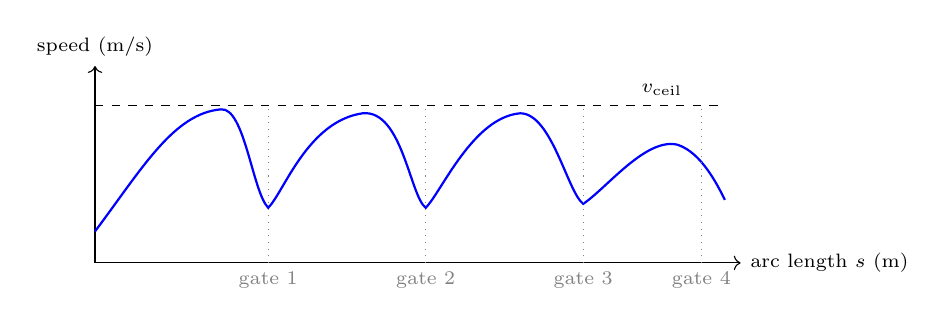
\begin{tikzpicture}[scale=1.0]
\draw[->] (0,0) -- (8.2,0) node[right, font=\scriptsize] {arc length $s$ (m)};
\draw[->] (0,0) -- (0,2.5) node[above, font=\scriptsize] {speed (m/s)};
\draw[dashed] (0,2.0) -- (8,2.0) node[pos=0.9, above, font=\scriptsize] {$v_{\text{ceil}}$};
\draw[thick, blue]
  (0,0.4)
  .. controls (0.6,1.2) and (1.0,1.9) .. (1.6,1.95)
  .. controls (1.9,1.98) and (2.0,0.9) .. (2.2,0.7)
  .. controls (2.4,0.9) and (2.7,1.8) .. (3.4,1.9)
  .. controls (3.9,1.95) and (4.0,0.85) .. (4.2,0.7)
  .. controls (4.4,0.9) and (4.8,1.85) .. (5.4,1.9)
  .. controls (5.8,1.9) and (6.0,0.9) .. (6.2,0.75)
  .. controls (6.5,0.95) and (7.0,1.6) .. (7.4,1.5)
  .. controls (7.7,1.4) and (7.9,1.0) .. (8.0,0.8);
\foreach \x/\n in {2.2/1, 4.2/2, 6.2/3, 7.7/4} {
  \draw[gray, dotted] (\x,0) -- (\x,2.0);
  \node[font=\scriptsize, gray] at (\x,-0.22) {gate \n};
}
\end{tikzpicture}%
}
\caption{Speed profile along the racing line. The speed is high on the straights and drops at each gate and tight turn, set by the shared acceleration budget of \eqref{eq:curv}--\eqref{eq:bwd}.}
\label{fig:speed}
\end{figure}

\subsection{Feedforward and PD Tracking}
\label{sec:track}
The tracker turns the current reference into an acceleration command. Let $p_r$, $v_r$ and $a_r$ be the reference position, velocity and acceleration at the current clock index, and let $p$ and $v$ be the measured position and velocity. The command is
\begin{equation}
a_{\text{cmd}} = a_r + K_p\,(p_r - p) + K_d\,(v_r - v).
\label{eq:pd}
\end{equation}
The feedforward term $a_r$ carries the planned motion. The PD term corrects the error that the model and the onboard layer leave. The reference velocity $v_r$ also carries the motion of the warp, so the drone follows the reference point as it slides onto a revealed gate. Near a gate we raise the gains $K_p$ and $K_d$, so the drone is held on the line where it matters most. The command is clipped to a maximum acceleration, then turned into a collective thrust and an attitude command by
\begin{equation}
f = m\,(a_{\text{cmd}} + g),
\label{eq:thrust}
\end{equation}
with $m$ the mass and $g$ the gravity vector. The onboard controller tracks that attitude and thrust. This is a geometric tracking law of the kind used for quadrotors \cite{lee}.

\subsection{Reacting to the Reveal: Warping the Line}
\label{sec:warp}
The line is built on the nominal gates. When a gate is revealed the true position differs, so the line has to move. We do not rebuild it. We warp the stored line, which is cheap and keeps the shape the speed profile was built for. The warp has three parts, shown in Fig.~\ref{fig:warp}.

The first part is a shift. Each gate $j$ stores the measured offset $\delta_j$ between its true and nominal center. A reference point that sits between the crossing index of gate $j$ and gate $j{+}1$ is shifted by a blend of the two offsets,
\begin{equation}
\hat p(k) = p_r(k) + (1-w)\,\delta_j + w\,\delta_{j+1}, \quad w = \frac{k - k_j}{k_{j+1} - k_j},
\label{eq:blend}
\end{equation}
with $k_j$ the clock index at which the line crosses gate $j$. The whole line slides to follow the revealed gates, and the blend keeps it smooth between them.

The second part is obstacle push-out. Each revealed obstacle is a vertical pole at $o$ with a safety radius $r_o$. If a point falls inside that radius, we move it straight out to the edge,
\begin{equation}
\hat p \leftarrow o + (\hat p - o)\,\frac{r_o}{\lVert \hat p - o \rVert} \quad \text{if } \lVert \hat p - o \rVert < r_o,
\label{eq:pushout}
\end{equation}
in the ground plane. The third part is the same rule for the two posts of each gate frame. Away from the crossing we keep the line clear of the posts, so the drone does not clip a frame that has rotated. Inside the crossing window we leave the line alone, so the drone goes through the opening and not around it.

\begin{figure}[t]
\centering
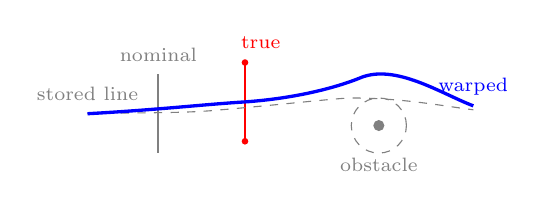
\begin{tikzpicture}[scale=1.0, font=\scriptsize]
\draw[gray, thick] (0.6,1.2) -- (0.6,0.2);
\node[gray] at (0.6,1.45) {nominal};
\draw[red, thick] (1.7,1.35) -- (1.7,0.35);
\node[red] at (1.9,1.6) {true};
\fill[red] (1.7,1.35) circle (1.2pt);
\fill[red] (1.7,0.35) circle (1.2pt);
\fill[gray] (3.4,0.55) circle (2pt);
\draw[gray, dashed] (3.4,0.55) circle (0.35);
\node[gray] at (3.4,0.05) {obstacle};
\draw[gray, dashed] (-0.3,0.7) .. controls (0.4,0.72) and (0.9,0.7) .. (1.4,0.75)
  .. controls (2.2,0.82) and (2.9,0.9) .. (3.05,0.9)
  .. controls (3.7,0.9) and (4.2,0.8) .. (4.6,0.75);
\node[gray] at (-0.3,0.95) {stored line};
\draw[blue, very thick] (-0.3,0.7)
  .. controls (0.6,0.75) and (1.2,0.82) .. (1.7,0.85)
  .. controls (2.4,0.9) and (2.9,1.05) .. (3.15,1.15)
  .. controls (3.6,1.35) and (4.2,0.95) .. (4.6,0.8);
\node[blue] at (4.6,1.05) {warped};
\end{tikzpicture}
\caption{Warping the stored line (dashed) onto the reveal (solid). The line slides onto the true gate opening and bows around the revealed obstacle. The shape is kept, only the position moves.}
\label{fig:warp}
\end{figure}

\subsection{The Adaptive Clock}
\label{sec:clock}
The reference is a list of points indexed by a clock. In normal flight the clock steps once per control tick, so the drone flies the line at the planned speed. A fixed clock has a weakness at a gate. If the gate has moved and the drone has to correct, a fixed clock keeps moving the reference forward while the drone is still catching up. The drone then reaches the gate plane behind its reference and off center, and it can clip the frame.

We make the clock adaptive, shown in Algorithm~\ref{alg:clock}. Near a gate the controller checks the gap between the drone and its current reference point. If the gap is large the clock stops and waits, up to a limit. If the gap is moderate the clock runs at two thirds speed. Otherwise it runs at full speed. Fig.~\ref{fig:clock} shows the effect. The clock stretches like a rubber band near a gate and returns to full speed once the drone is back on the line. When the clock is stopped the feedforward terms are set to zero, so the PD law pulls the drone onto the fixed reference point. This is the part that lets a fast line stay reliable. The drone never commits to a gate crossing faster than it can hold the opening.

\begin{algorithm}[t]
\caption{Adaptive clock update (one control tick)}
\label{alg:clock}
\begin{algorithmic}[1]
\REQUIRE clock index $k$, drone position $p$, next gate center $g$
\STATE $e \leftarrow \lVert \hat{p}(k) - p \rVert$ \quad (gap to the reference point)
\STATE $\mathit{near} \leftarrow \lVert p - g \rVert < 1.2$
\IF{$\mathit{near}$ and $e \ge 0.22$}
    \STATE \textsc{freeze}: keep $k$ this tick, for at most 75 ticks
\ELSIF{$\mathit{near}$ and $0.14 \le e < 0.22$}
    \STATE \textsc{slow}: advance $k$ on two of every three ticks
\ELSE
    \STATE \textsc{run}: $k \leftarrow k + 1$
\ENDIF
\end{algorithmic}
\end{algorithm}

\begin{figure}[t]
\centering
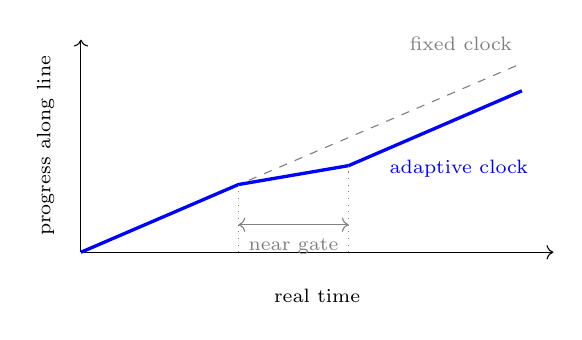
\begin{tikzpicture}[font=\scriptsize]
% axes
\draw[->] (0,0) -- (6.0,0);
\node at (3.0,-0.55) {real time};
\draw[->] (0,0) -- (0,2.7);
\node[rotate=90] at (-0.45,1.35) {progress along line};
% fixed clock: constant rate
\draw[gray, dashed] (0,0) -- (5.6,2.4);
\node[gray, anchor=south east] at (5.6,2.44) {fixed clock};
% adaptive clock: same rate, slow near the gate, then same rate (now lagging behind)
\draw[blue, very thick] (0,0) -- (2.0,0.86) -- (3.4,1.10) -- (5.6,2.05);
\node[blue, anchor=north] at (4.8,1.30) {adaptive clock};
% gate window
\draw[gray, dotted] (2.0,0) -- (2.0,0.86);
\draw[gray, dotted] (3.4,0) -- (3.4,1.10);
\draw[<->, gray] (2.0,0.35) -- (3.4,0.35);
\node[gray, anchor=north] at (2.7,0.30) {near gate};
\end{tikzpicture}
\caption{The adaptive clock. A fixed clock (dashed) advances the reference at a constant rate. The adaptive clock (solid) slows or stops near a gate while the drone catches up, then returns to full speed.}
\label{fig:clock}
\end{figure}

\subsection{Launch}
The start is handled by a short vertical climb. The rotors spin up from rest, and the environment disables the drone on any floor touch once it drifts from the start pad. A fixed low climb holds the start position through that window. Control then passes to the tracker, which builds the racing line from the current state with the current velocity direction, so the drone leaves the climb along the line.

\section{Evaluation and Results}
\label{sec:results}

\subsection{Setup}
We evaluate on the \texttt{final.toml} competition track of Section~\ref{sec:problem}, the fixed-layout course that every group shares. Its nominal layout of four gates and four obstacles is shown in Fig.~\ref{fig:track}. The line reverses direction twice, once near the third gate and once before the last gate, which set the pace. The reported numbers are from the official evaluation with seed 2026, which draws a fresh disturbance for each of the 20 runs. Table~\ref{tab:params} lists the main parameters. They are tuned once offline and are held fixed across all runs.

\begin{figure}[t]
\centering
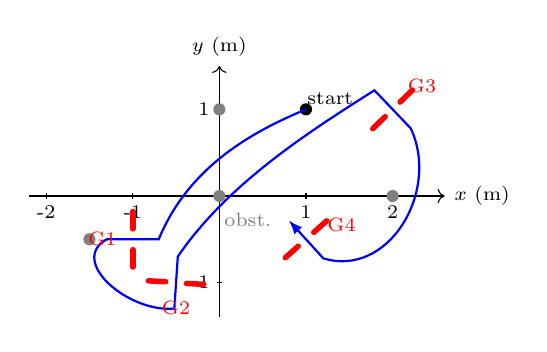
\begin{tikzpicture}[scale=1.1, font=\scriptsize,
  post/.style={red, line width=2pt, line cap=round}]
% axes
\draw[->] (-2.2,0) -- (2.6,0) node[right] {$x$ (m)};
\draw[->] (0,-1.4) -- (0,1.5) node[above] {$y$ (m)};
\foreach \x in {-2,-1,1,2} \draw (\x,-0.03) -- (\x,0.03) node[below=1pt] {\x};
\foreach \y in {-1,1} \draw (-0.03,\y) -- (0.03,\y) node[left=1pt] {\y};
% obstacles and start
\foreach \ox/\oy in {0/0, -1.5/-0.5, 0/1.0, 2.0/0} { \fill[gray] (\ox,\oy) circle (2pt); }
\node[gray] at (0.33,-0.27) {obst.};
\fill[black] (1.0,1.0) circle (2pt); \node at (1.28,1.13) {start};
% racing line: start -> G1 -> G2 -> G3 -> G4.
% straight segments cross each gate through the gap; curves connect the gates.
\draw[blue, thick, -{Latex[length=1.8mm]}]
  (1.0,1.0)
  .. controls (0.4,0.75) and (-0.35,0.35) .. (-0.70,-0.50) % start -> G1 entry
  -- (-1.30,-0.50)                                          % cross G1
  .. controls (-1.75,-0.75) and (-1.05,-1.35) .. (-0.52,-1.30) % -> G2 entry
  -- (-0.48,-0.70)                                          % cross G2
  .. controls (0.10,0.15) and (1.05,0.75) .. (1.79,1.22)   % -> G3 entry
  -- (2.21,0.78)                                            % cross G3
  .. controls (2.55,0.05) and (1.95,-0.95) .. (1.20,-0.72) % -> G4 entry
  -- (0.80,-0.28);                                          % cross G4
% gates: two frame posts with the opening (gap) between them
\draw[post] (-1.0,-0.18) -- (-1.0,-0.38);
\draw[post] (-1.0,-0.62) -- (-1.0,-0.82); \node[red] at (-1.35,-0.5) {G1};
\draw[post] (-0.18,-1.02) -- (-0.38,-1.01);
\draw[post] (-0.62,-0.99) -- (-0.82,-0.98); \node[red] at (-0.5,-1.29) {G2};
\draw[post] (1.914,0.916) -- (1.771,0.777);
\draw[post] (2.086,1.084) -- (2.229,1.223); \node[red] at (2.34,1.27) {G3};
\draw[post] (0.910,-0.580) -- (0.761,-0.713);
\draw[post] (1.090,-0.420) -- (1.239,-0.287); \node[red] at (1.41,-0.33) {G4};
\end{tikzpicture}
\caption{Nominal layout of the competition track (top view, \texttt{final.toml}). Each gate is drawn as its two frame posts with the opening between them, numbered G1 to G4 in pass order. Grey dots are obstacles and the blue line is the racing line built offline on this layout. Each run shifts every gate and obstacle from its nominal pose by up to 0.15 m, which the controller corrects online. The line reverses near G3 and before G4.}
\label{fig:track}
\end{figure}


\begin{table}[htbp]
\caption{Main controller parameters}
\begin{center}
\begin{tabular}{|l|c|}
\hline
\textbf{Parameter} & \textbf{Value} \\
\hline
Top speed cap $v_{\text{ceil}}$ & 3.8 m/s \\
\hline
Turning budget $a_{\text{lat}}$ & 8.5 m/s\textsuperscript{2} \\
\hline
Forward / brake budget $a_H$ / $a_B$ & 6.5 / 4.5 m/s\textsuperscript{2} \\
\hline
Gate speed caps & 1.8, 2.4, 2.4, 2.4 m/s \\
\hline
Gate cap radius & 0.40 m \\
\hline
Tracking gains $K_p$ / $K_d$ & 8--10 / 6--7 \\
\hline
Gate gains $K_p$ / $K_d$ & 24--26 / 10--11 \\
\hline
Command accel limit & 14 m/s\textsuperscript{2} \\
\hline
Control rate & 50 Hz \\
\hline
\end{tabular}
\label{tab:params}
\end{center}
\end{table}

\subsection{Main Result}
On the official evaluation the controller passes all 20 runs with a lap time of 6.89 s. Fig.~\ref{fig:screenshot} shows a run. All four gates are crossed near their centers, and the drone stays clear of the obstacles and the frame posts. The controller holds the 50 Hz rate with a wide margin, since it runs no solver and only evaluates the warp and the tracking law each step.

\begin{figure}[t]
\centering
\figplaceholder{42mm}{Simulation screenshot or flown-trajectory overlay.\\ Suggested: a top-down plot of the planned line and the\\ actual paths over the 20 runs, or a render of the drone\\ passing a gate. Replace with \texttt{\textbackslash includegraphics}.}
\caption{A run on the Level 3 track. \textcolor{red}{[Insert a simulation screenshot or a trajectory plot here.]}}
\label{fig:screenshot}
\end{figure}

\subsection{Comparison with the Optimization Controller}
Before this controller we built an online Model Predictive Contouring Control controller for the same track, and we flew it on the real Crazyflie in the last lab session (Section~\ref{sec:deploy}). Table~\ref{tab:compare} compares the two in simulation. The optimization controller reaches 9.55 s and needs a compiled solver in the loop. The feedforward tracker is 2.66 s faster and passes all runs, and it has no solver, so it is simpler to run and to reason about. The gain does not come from a faster vehicle. Both use the same drone and the same acceleration limits. It comes from where the effort goes. The optimization controller spends the run re-solving a hard problem near each gate, while the tracker spends it holding a fixed line with a clock that waits when needed.

\begin{table}[htbp]
\caption{Comparison on the Level 3 track}
\begin{center}
\begin{tabular}{|l|c|c|c|}
\hline
\textbf{Controller} & \textbf{Solver} & \textbf{Success} & \textbf{Lap (s)} \\
\hline
Online MPCC & yes & --$^{\mathrm{a}}$ & 9.55$^{\mathrm{a}}$ \\
\hline
Feedforward tracker (ours) & no & 20/20 & 6.89 \\
\hline
\multicolumn{4}{l}{$^{\mathrm{a}}$best lap; full success rate not recorded on this track.}
\end{tabular}
\label{tab:compare}
\end{center}
\end{table}

\subsection{Effect of Each Part}
Table~\ref{tab:ablation} shows how the result changed as we added each part, measured on the official evaluation. The base is the adaptive clock with the obstacle and gate-post push-out. It reached 19 of 20 at 7.13 s. The one failure was a gate that had moved far, where the clock only had a stop-or-go choice and the correction was abrupt. Running the clock at two thirds speed near a gate, rather than only stop or go, smoothed the correction and cut the time to 6.92 s at the same success. Tuning the turning budget and the gate cap radius recovered the last run and reached 20 of 20 at 6.89 s. A plot of the tracking gap against the clock state over a run would show where the clock slows, and it is a good candidate for the space in Fig.~\ref{fig:screenshot}.

\begin{table}[htbp]
\caption{Effect of each part on the official evaluation}
\begin{center}
\begin{tabular}{|l|c|c|}
\hline
\textbf{Configuration} & \textbf{Success} & \textbf{Lap (s)} \\
\hline
Adaptive clock + push-out & 19/20 & 7.13 \\
\hline
+ two-thirds-rate clock & 19/20 & 6.92 \\
\hline
+ tuned budget and gate radius & 20/20 & 6.89 \\
\hline
\end{tabular}
\label{tab:ablation}
\end{center}
\end{table}

\subsection{Why This Works}
The design splits the problem into a shape and a timing. The shape is the racing line, built once and warped onto the reveal, so the drone always has a smooth curve to follow. The timing is the adaptive clock, which holds the drone back near a gate until it is on the line. An online optimizer folds these into one problem and pays for it with a solver at every step and with the risk of a hard step near a gate. Splitting them keeps each part simple and lets us tune them on their own. The reveal is handled by the warp and the clock, not by a new plan, so the drone never faces a fresh and sharp trajectory in the middle of a fast approach. This also explains the low run-to-run spread. The line is the same every run, and only the small warp and the clock differ with the draw.

\section{From Simulation to the Real World}
\label{sec:deploy}
This line of work has already flown on real hardware. In the last lab session we flew the predecessor of the tracker, an online Model Predictive Contouring Control controller, on the physical Crazyflie under the Vicon system. It completed the course with a lap time of 9.55 s, and its behaviour on the drone matched its simulation. This tells us that the simulator we use is a good proxy for the real vehicle on this track.

The tracker in this report was built after that session as an improvement. It reaches 6.89 s at 20 of 20 runs in simulation and has not yet been flown. Two reasons support a transfer. The simulator matched the real flight for the predecessor, and the tracker is the simpler of the two controllers. It runs no solver and has a fixed per-step cost, so the 50 Hz rate is safe on modest hardware. The control law is a feedforward term with a PD correction, which is standard on quadrotors and does not depend on an exact model.

The main residual risk is the gap between the simulated and the real dynamics. The feedforward acceleration assumes the onboard controller tracks the attitude command quickly, and the real mass and thrust differ from the nominal values. A common fix is to scale the speed and the acceleration budget down by a small factor, which trades a little lap time for margin. The gate speed caps already give some of that margin at the point where it matters most. A short set of hover and step tests on the real vehicle would set the scale factor before a full run.

\section{Limitations and Future Work}
\label{sec:limits}
The controller has three limits worth naming. First, the warp shifts the line for a gate that has moved, but it does not re-aim the crossing for a gate that has rotated. A large yaw change is only handled by the post push-out, which keeps the drone clear of the frame but does not re-center the approach. Warping the line for the revealed yaw is the clear next step. Second, the line is built once on the nominal course. It assumes the gate order and the rough layout hold. A very large shift that changes the topology would need a reshape, which the warp does not do. Third, the offsets and the leg control points are tuned for this track. A new track needs the offline line built again, though the tracker and the clock stay the same. Future work is to warp the yaw, to fit the offline offsets with a short search rather than by hand and to test the controller on the real vehicle.

\section{Conclusion}
We presented a controller for autonomous drone racing under disturbance that runs no optimizer in the loop. A time-optimal racing line is built once from the nominal course and tracked with a feedforward term and a PD law. When a gate is revealed the stored line is slid onto the true gate and pushed clear of obstacles, and the drone flies the line by an adaptive clock that slows near a gate when the drone falls behind. On the competition track the controller passes all 20 evaluation runs in simulation at 6.89 s. The earlier controller in this line flew on the real drone at 9.55 s and matched its simulation there, so we expect the tracker's gains to hold on hardware. The design keeps the shape and the timing separate, which makes each part simple to tune and keeps the run-to-run spread small.

\appendices
\section{Reproducibility}
The controller is evaluated on the \texttt{final.toml} Level 3 track with seed 2026 in the LSY Drone Racing environment, in attitude control mode at 50 Hz, with the Crazyflie 2.1 model. The offline line, the speed profile and the tracking law use the values in Table~\ref{tab:params}. The gate speed caps, the entry and exit offsets and the leg control points are the only track-specific values. All other parameters are shared across tracks. The controller code is in the project repository.

\begin{thebibliography}{00}
\bibitem{survey} D. Hanover, A. Loquercio, L. Bauersfeld, A. Romero, R. Penicka, Y. Song, G. Cioffi, E. Kaufmann, and D. Scaramuzza, ``Autonomous drone racing: A survey,'' IEEE Trans. Robot., vol. 40, pp. 3044--3067, 2024.
\bibitem{foehn} P. Foehn, A. Romero, and D. Scaramuzza, ``Time-optimal planning for quadrotor waypoint flight,'' Sci. Robot., vol. 6, no. 56, 2021.
\bibitem{minsnap} D. Mellinger and V. Kumar, ``Minimum snap trajectory generation and control for quadrotors,'' in IEEE Int. Conf. Robotics and Automation (ICRA), 2011, pp. 2520--2525.
\bibitem{kunz} T. Kunz and M. Stilman, ``Time-optimal trajectory generation for path following with bounded acceleration and velocity,'' in Robotics: Science and Systems (RSS), 2012.
\bibitem{verscheure} D. Verscheure, B. Demeulenaere, J. Swevers, J. De Schutter, and M. Diehl, ``Time-optimal path tracking for robots: A convex optimization approach,'' IEEE Trans. Autom. Control, vol. 54, no. 10, pp. 2318--2327, 2009.
\bibitem{mpcc} A. Romero, S. Sun, P. Foehn, and D. Scaramuzza, ``Model predictive contouring control for time-optimal quadrotor flight,'' IEEE Trans. Robot., vol. 38, no. 6, pp. 3340--3356, 2022.
\bibitem{lee} T. Lee, M. Leok, and N. H. McClamroch, ``Geometric tracking control of a quadrotor UAV on SE(3),'' in IEEE Conf. Decision and Control (CDC), 2010, pp. 5420--5425.
\bibitem{scg} Z. Yuan, A. W. Hall, S. Zhou, L. Brunke, M. Greeff, J. Panerati, and A. P. Schoellig, ``Safe-control-gym: a unified benchmark suite for safe learning-based control and reinforcement learning in robotics,'' IEEE Robot. Autom. Lett., vol. 7, no. 4, pp. 11142--11149, 2022.
\bibitem{crazyflie} W. Giernacki, M. Skwierczy\'nski, W. Witwicki, P. Wro\'nski, and P. Kozierski, ``Crazyflie 2.0 quadrotor as a platform for research and education in robotics and control engineering,'' in Int. Conf. Methods and Models in Automation and Robotics (MMAR), 2017, pp. 37--42.
\bibitem{champion} E. Kaufmann, L. Bauersfeld, A. Loquercio, M. M\"uller, V. Koltun, and D. Scaramuzza, ``Champion-level drone racing using deep reinforcement learning,'' Nature, vol. 620, pp. 982--987, 2023.
\bibitem{songrl} Y. Song, M. Steinweg, E. Kaufmann, and D. Scaramuzza, ``Autonomous drone racing with deep reinforcement learning,'' in IEEE/RSJ Int. Conf. Intelligent Robots and Systems (IROS), 2021, pp. 1205--1212.
\end{thebibliography}

\end{document}
